\documentclass[a4paper,12pt]{extarticle}
\usepackage[utf8x]{inputenc}
\usepackage[T1,T2A]{fontenc}
\usepackage[russian]{babel}
\usepackage{hyperref}
\usepackage{indentfirst}
\usepackage{listings}
\usepackage{color}
\usepackage{here}
\usepackage{array}
\usepackage{multirow}
\usepackage{graphicx}

\usepackage{caption}
\renewcommand{\lstlistingname}{Программа} % заголовок листингов кода

\bibliographystyle{ugost2008ls}

\usepackage{listings}
\lstset{ %
extendedchars=\true,
keepspaces=true,
language=C,						% choose the language of the code
basicstyle=\footnotesize,		% the size of the fonts that are used for the code
numbers=left,					% where to put the line-numbers
numberstyle=\footnotesize,		% the size of the fonts that are used for the line-numbers
stepnumber=1,					% the step between two line-numbers. If it is 1 each line will be numbered
numbersep=5pt,					% how far the line-numbers are from the code
backgroundcolor=\color{white},	% choose the background color. You must add \usepackage{color}
showspaces=false				% show spaces adding particular underscores
showstringspaces=false,			% underline spaces within strings
showtabs=false,					% show tabs within strings adding particular underscores
frame=single,           		% adds a frame around the code
tabsize=2,						% sets default tabsize to 2 spaces
captionpos=t,					% sets the caption-position to top
breaklines=true,				% sets automatic line breaking
breakatwhitespace=false,		% sets if automatic breaks should only happen at whitespace
escapeinside={\%*}{*)},			% if you want to add a comment within your code
postbreak=\raisebox{0ex}[0ex][0ex]{\ensuremath{\color{red}\hookrightarrow\space}},
texcl=true,
inputpath=listings,                     % директория с листингами
}

\usepackage[left=2cm,right=2cm,
top=2cm,bottom=2cm,bindingoffset=0cm]{geometry}

%% Нумерация картинок по секциям
\usepackage{chngcntr}
\counterwithin{figure}{section}
\counterwithin{table}{section}

%%Точки нумерации заголовков
\usepackage{titlesec}
\titlelabel{\thetitle.\quad}
\usepackage[dotinlabels]{titletoc}

%% Оформления подписи рисунка
\addto\captionsrussian{\renewcommand{\figurename}{Рисунок}}
\captionsetup[figure]{labelsep = period}

%% Подпись таблицы
\DeclareCaptionFormat{hfillstart}{\hfill#1#2#3\par}
\captionsetup[table]{format=hfillstart,labelsep=newline,justification=centering,skip=-10pt,textfont=bf}

%% Путь к каталогу с рисунками
\graphicspath{{fig/}}


\begin{document}	% начало документа

% Титульная страница
\begin{titlepage}	% начало титульной страницы

	\begin{center}		% выравнивание по центру

		\large Санкт-Петербургский Политехнический Университет Петра Великого\\
		\large Институт компьютерных наук и технологий \\
		\large Кафедра компьютерных систем и программных технологий\\[6cm]
		% название института, затем отступ 6см
		
		\huge Сети и телекоммуникации\\[0.5cm] % название работы, затем отступ 0,5см
		\large Отчет по лабораторной работе №1\\[0.1cm]
		\large Программирование сокетов протоколов TCP и UDP\\[5cm]

	\end{center}


	\begin{flushright} % выравнивание по правому краю
		\begin{minipage}{0.25\textwidth} % врезка в половину ширины текста
			\begin{flushleft} % выровнять её содержимое по левому краю

				\large\textbf{Работу выполнил:}\\
				\large Коренёк Г.А.\\
				\large {Группа:} 43501/3\\
				
				\large \textbf{Преподаватель:}\\
				\large Алексюк А.О.

			\end{flushleft}
		\end{minipage}
	\end{flushright}
	
	\vfill % заполнить всё доступное ниже пространство

	\begin{center}
	\large Санкт-Петербург\\
	\large \the\year % вывести дату
	\end{center} % закончить выравнивание по центру

\thispagestyle{empty} % не нумеровать страницу
\end{titlepage} % конец титульной страницы

\vfill % заполнить всё доступное ниже пространство


% Содержание
% Содержание
\renewcommand\contentsname{\centerline{Содержание}}
\tableofcontents
\newpage




\section{Цель работы}

Изучение принципов программирования сокетов протоколов TCP и UDP.

\section{Программа работы}

\begin{itemize}
\item разработать простейший клиент и сервер на основе протоколов TCP и UDP
\item разработать прикладной протокол в соответствии с индивидуальным заданием, реализовать протокол в виде клиент-серверного приложения на основе протоколов TCP и UDP
\item выполнить дополнительное задание
\end{itemize}

\section{Ход выполнения работы}

\subsection{Простейшие клиент и сервер}
Простейшие клиент и сервер были выполнены на основе протоколов TCP и UDP, а также адаптированы под ОС Windows и Linux. Сервер выполняет функции эхо-сервера, т.е. принимает сообщения от клиентов и посылает копии обратно. Клиент посылает сообщение, после чего завершается.

\subsection{Индивидуальное задание}

В качестве индивидуального задания была выбрана система обмена мгновенными сообщениями. Сервер реализован на Windows, клиент - на Linux.

Серверное приложение реализует следующие функции:
\begin{itemize}
\item Прослушивание определенного порта
\item Обработка запросов на подключение по этому порту от клиентов
\item Поддержка одновременной работы нескольких клиентов через механизм нитей
\item Передача текстового сообщения одному клиенту
\item Передача текстового сообщения всем клиентам
\item Прием и ретрансляция входящих сообщений от клиентов
\item Обработка запроса на отключение клиента
\item Принудительное отключение указанного клиента
\end{itemize}

Клиентское приложение реализует следующие функции:

\begin{itemize}
\item Установление соединения с сервером
\item Передача сообщения всем клиентам
\item Передача сообщения указанному клиенту
\item Прием сообщения от сервера с последующей индикацией
\item Разрыв соединения
\item Обработка ситуации отключения клиента сервером
\end{itemize}

Разработанное клиентское приложение предоставлет пользователю настройку IP-адреса или доменного имени сервера сообщений и номера порта сервера.

\subsubsection{Реализация на TCP}

Для реализации данной системы был разработан текстовый асинхронный протокол. Его схема для реализации на TCP представлена на рис. 3.1

\begin{figure}[H]
	\begin{center}
		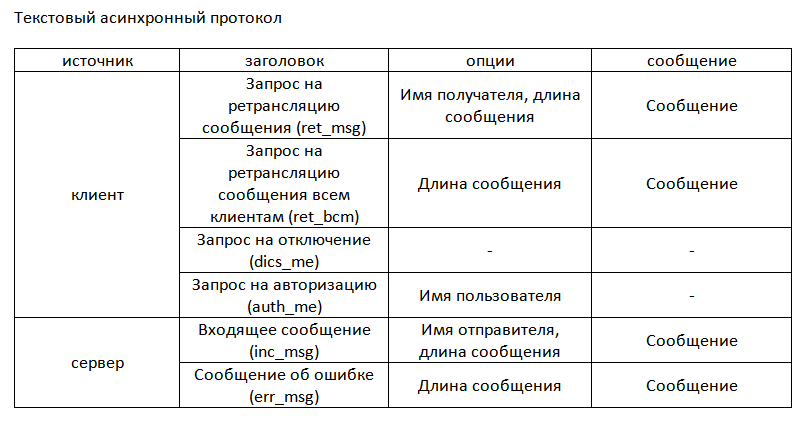
\includegraphics[scale=0.7]{protocol_tcp}
		\caption{Схема прикладного протокола для реализации на TCP} 
		\label{pic:pic_name} % название для ссылок внутри кода
	\end{center}
\end{figure}

\paragraph{Описание протокола:}

Сообщение всегда содержит, как минимум, поле заголовка, определяющее тип сообщения. Некоторые типы сообщений содержат также поле опций. Для типов сообщений, содержащих данные (собственно пользовательское сообщение), в поле опций, кроме прочего, указывается длина сообщения, чтобы принимающая сторона принимала нужное число символов.

Поле заголовка имеет фиксированный размер 8 байт. Поле опций может (в зависимости от заголовка) отсутствовать или содержать до 2 частей - имя пользователя и длину данных. Имя пользователя, в зависимости от заголовка, содержит имя получателя, отправителя или имя пользователя для авторизации. Эта часть поля опций занимает 16 байт. Часть поля опций, содержащая длину данных, занимает 2 байта, длина данных передается в бинарном виде. Поэтому максимальная длина поля данных составляет 16К символов (байт).

\paragraph{Описание программы:}

Сервер имеет 1 слушающий порт, по которому принимает от клиентов запросы на соединение. При подсоединении очередного клиента, для связи с ним выделяется отдельный сокет, прием из которого осуществляется в отдельном потоке. Для дальнейшего управления порожденными потоками (например, завершение потока при получении от клиента запроса на отключение) при подключении клиента осуществляется вставка в хэш-таблицу id его сокета в качестве ключа и id потока в качестве значения.

После подключения клиента сервер ожидает приема 8 символов заголовка. Допустимые значения заголовков хранятся в хэш-таблице в качестве ключа. В качестве значения в ней хранятся ссылки на функции-обработчики. При совпадении принятого заголовка с имеющимся в таблице происходит вызов соответствующего обработчика.

Обработчик, в зависимости от соответствующего типа сообщения, может содержать вызовы для приема оставшейся части сообщения - опций и данных.

Для управления сервером предусмотрен поток для опроса стандартного потока ввода. Его работа схожа с работой потока приема заголовков. Есть хэш-таблица с допустимыми командами в качестве ключа и обработчиками в качестве значения. При вводе команды вызывается обработччичк. Обработчик может считывать со стандартного ввода необходимые дополнения для введенных команд.

Принцип работы клиента схож с принципом работы сервера. Основное отличие в том, что имеется только 1 поток для приема сообщений. Список допустимых принимаемых заголовков для клиента совпадает со списком посылаемых сервером заголовков, и наоборот. Отличается также список команд, принимаемых с клавиатуры.

\subsubsection{Реализация на UDP}

\paragraph{Описание протокола:}

Реализация прикладного протокола на UDP схожа с реализацией на TCP. Протокол отличается тем, что теперь не передается длина сообщения, но перед заголовком передается порядковый номер сообщения. Размер поля номера сообщения составляет 4 байта, номер передается в бинарном виде.

\paragraph{Описание программы:}

В отличие от варианта TCP, здесь не происходит установления соединения и все сообщения передаются через один сокет.

Сервер использует хэш-таблицу, в которой хранится сетевой адрес клиента(ключ) и соответствующий ему номер последнего принятого (в другой таблице -- отправленного) сообщения. При приеме (отправке) очередного сообщения его номер сравнивается с содержимым соответствующей таблицы, и, в случае нарушения порядка следования пакетов, сообщение об этом выводится в консоль.

\subsection{Дополнительное задание}

В качестве дополнительного задания необходимо исследовать реальные прикладные протоколы. Необходимо "притвориться" клиентом и подключиться к одному из существующих общедоступных серверов.

В качестве утилиты для подключения к серверам была выбрана telnet.

\subsubsection{Подключение к веб-серверу и запрос веб-страницы}

Был произведен запрос веб-страницы с сервера tiger.ftk.spbstu.ru (рис. 3.2) Подключение производится по используемому протоколом http порту 80. Сервер вернул код 200 в заголовке ответа, что говорит об успешной обработке запроса.

\begin{figure}[H]
	\begin{center}
		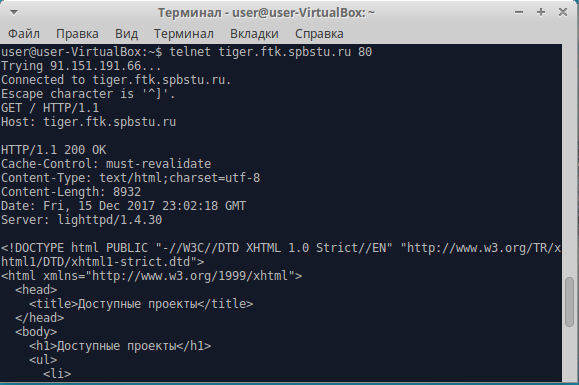
\includegraphics[scale=0.7]{http}
		\caption{Запрос веб-страницы} 
		\label{pic:pic_name} % название для ссылок внутри кода
	\end{center}
\end{figure}

\subsubsection{Запрос списка файлов и загрузка файла с ftp-сервера}

Протокол FTP использует 2 соединения - для передачи команд и для передачи данных. Поэтому подключение к нему производится в 2 этапа: сначала производится подключение к порту 21 (для передачи команд) и авторизация, затем переход в пассивный режим и подключение из другого терминала к порту, указанному сервером (рис. 3.3 - 3.4)

\begin{figure}[H]
	\begin{center}
		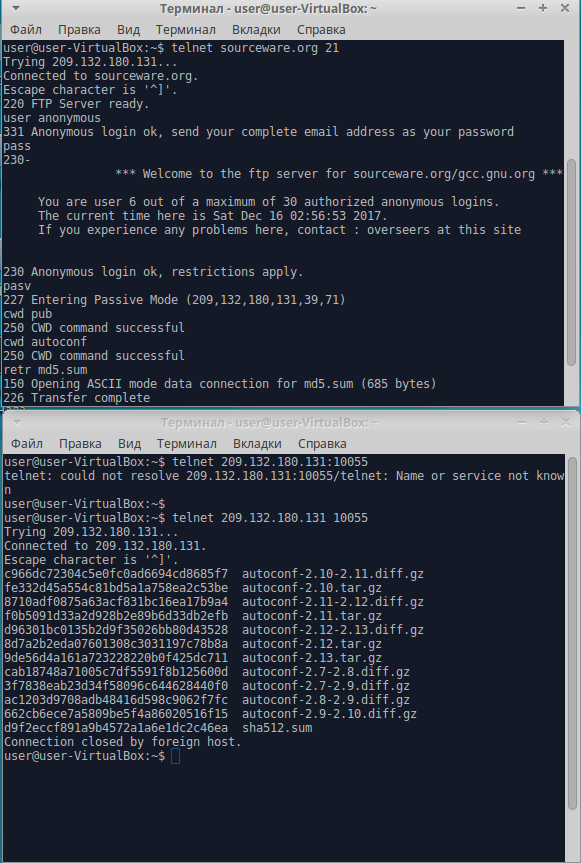
\includegraphics[scale=0.7]{ftp1}
		\caption{Запрос списка файлов и загрузка файла с ftp-сервера} 
		\label{pic:pic_name} % название для ссылок внутри кода
	\end{center}
\end{figure}

\begin{figure}[H]
	\begin{center}
		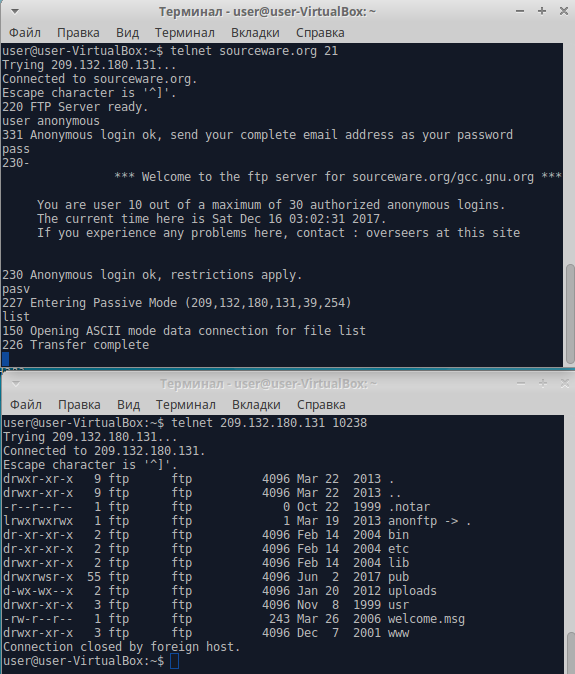
\includegraphics[scale=0.7]{ftp2}
		\caption{Запрос списка файлов и загрузка файла с ftp-сервера} 
		\label{pic:pic_name} % название для ссылок внутри кода
	\end{center}
\end{figure}

\subsubsection{Отправка письма на SMTP-сервер}

Попытаемся авторизоваться на SMTP-сервере gmail  (рис. 3.5)

\begin{figure}[H]
	\begin{center}
		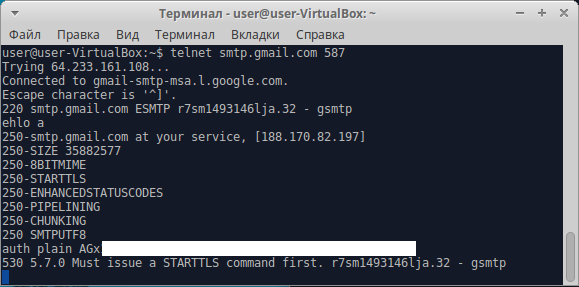
\includegraphics[scale=0.7]{smtp0}
		\caption{Отправка письма на SMTP-сервер без использования шифрования} 
		\label{pic:pic_name} % название для ссылок внутри кода
	\end{center}
\end{figure}

Как видно, данный сервер требует обязательного использования TLS. Установим защищенное соединение с помощью утилиты openssl (рис. 3.6 - 3.7)

\begin{figure}[H]
	\begin{center}
		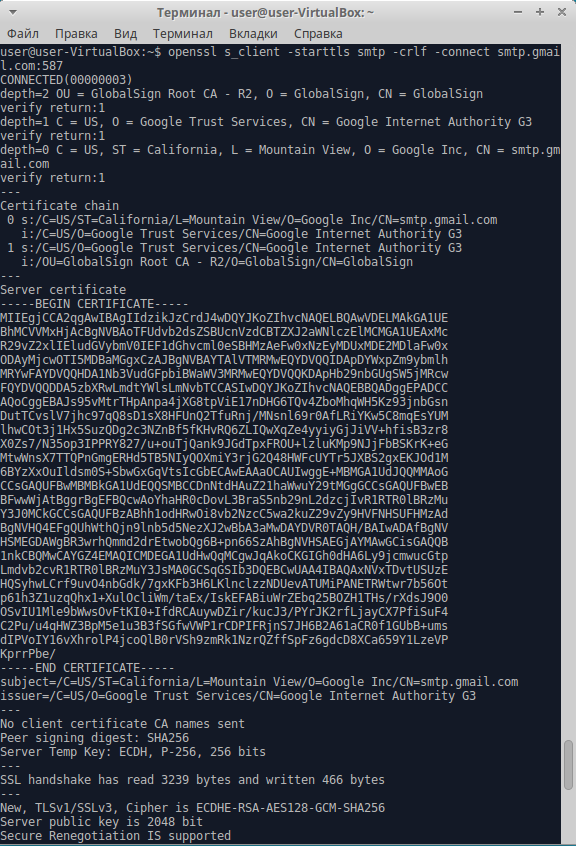
\includegraphics[scale=0.7]{smtp1}
		\caption{Отправка письма на SMTP-сервер через TLS-подключение}
		\label{pic:pic_name} % название для ссылок внутри кода
	\end{center}
\end{figure}

\begin{figure}[H]
	\begin{center}
		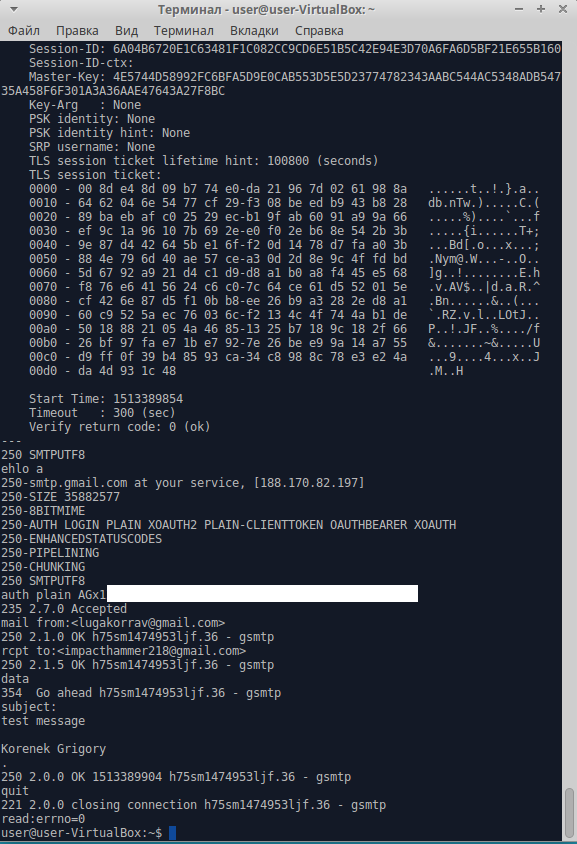
\includegraphics[scale=0.7]{smtp2}
		\caption{Отправка письма на SMTP-сервер через TLS-подключение} 
		\label{pic:pic_name} % название для ссылок внутри кода
	\end{center}
\end{figure}

Сервер сообщил, что сообщение успешно отправлено. Убедимся в этом, зайдя на gmail.com (рис. 3.8)

\begin{figure}[H]
	\begin{center}
		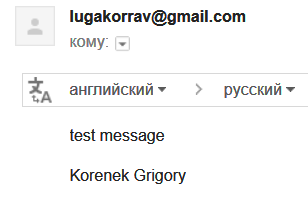
\includegraphics[scale=0.7]{smtp3}
		\caption{Отправленое письмо} 
		\label{pic:pic_name} % название для ссылок внутри кода
	\end{center}
\end{figure}

\subsubsection{Получение письма с POP3-сервера}

Проверим почту и получим письмо (рис. 3.9 - 3.11)

\begin{figure}[H]
	\begin{center}
		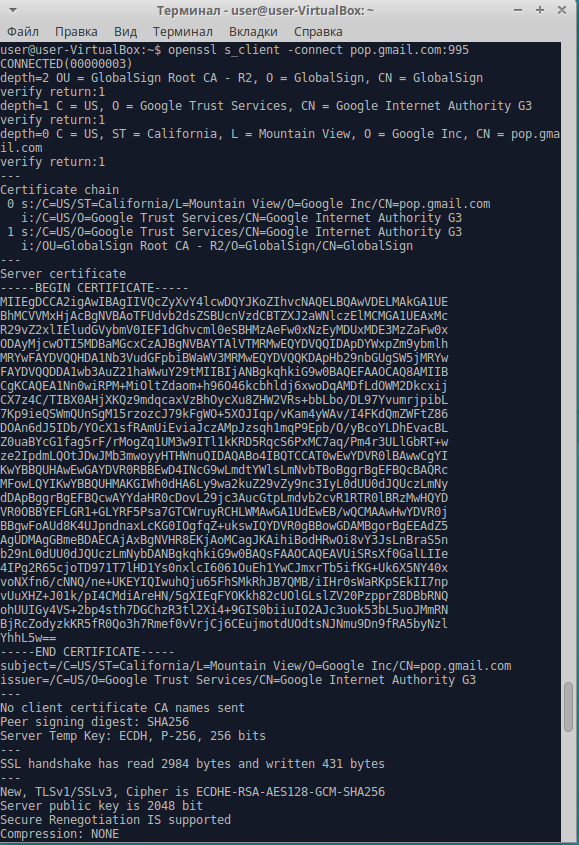
\includegraphics[scale=0.7]{pop3_1}
		\caption{Получение письма с POP3-сервера} 
		\label{pic:pic_name} % название для ссылок внутри кода
	\end{center}
\end{figure}

\begin{figure}[H]
	\begin{center}
		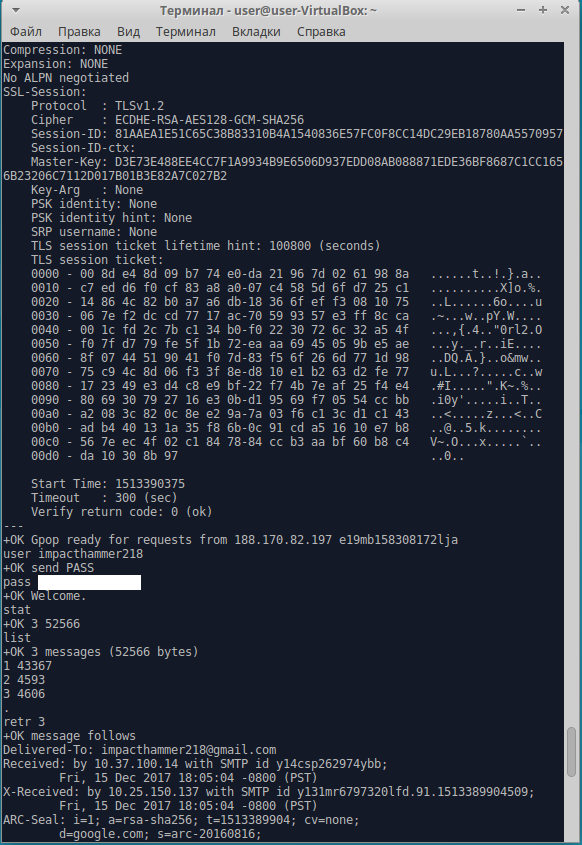
\includegraphics[scale=0.7]{pop3_2}
		\caption{Получение письма с POP3-сервера} 
		\label{pic:pic_name} % название для ссылок внутри кода
	\end{center}
\end{figure}

\begin{figure}[H]
	\begin{center}
		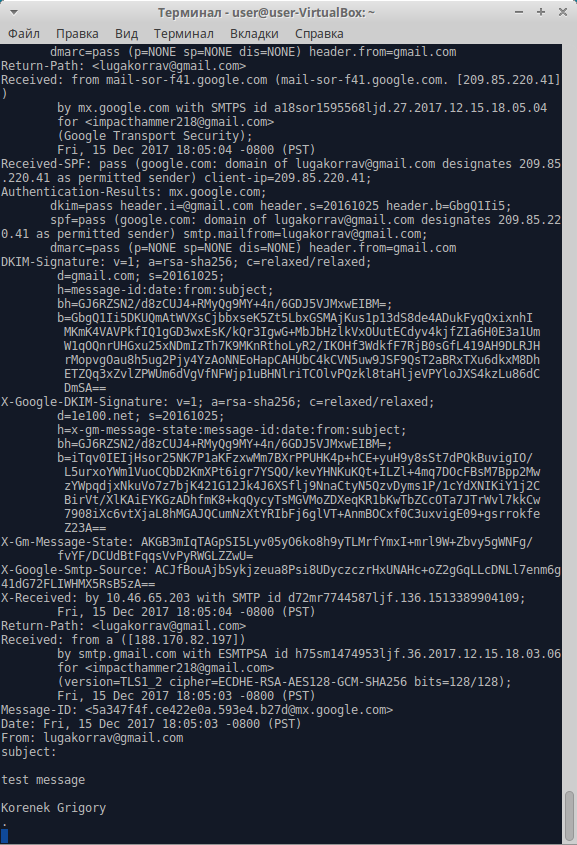
\includegraphics[scale=0.7]{pop3_3}
		\caption{Получение письма с POP3-сервера} 
		\label{pic:pic_name} % название для ссылок внутри кода
	\end{center}
\end{figure}

\section{Выводы}

В ходе работы был разработан и реализован в виде приложения прикладной протокол. В результате этого были изучены принципы программирования сокетов TCP и UDP. Основной проблемой при реализации приложения на TCP была необходимость контроля длины посылки. Ее решением стало добавление длины посылки в поле опций. После приема посылки принимающая сторона ожидает приема указанного числа символов. Проблема контроля потоков опроса клиентов решилась сохранением в хэш-таблице сокетов клиентов и соответствующих id потоков. TCP требует установления соединения, поэтому на сервере выделяется поток, в котором происходит прием запросов на соединение от клиентов через выделенный для этого сокет. После подключения очередного клиента порождается отдельный поток, осуществляющий обмен пакетами с этим клиентом через отдельный сокет. Этот поток принимает заголовок сообщения, после чего вызывает соответствующий обработчик. Обработчик, если требуется, принимает опции и данные и выполняет необходимые действия по обработке сообщения. Подобным образом работает и обработка команд с клавиатуры.

При реализации на UDP требовалось определять ситуации перемешивания и потери пакетов. Для этого на сервере создавались хэш-таблицы, хранящие адреса клиентов (ключи) и соответствующие номера отправляемых (принимаемых) пакетов. Для клиента с этой целью требовалось хранить только 2 переменные. В реализации на UDP сервер обменивается пакетами со всеми клиентами в одном потоке и через один сокет, т.к. нет установления соединения.

Также были исследованы прикладные протоколы. Как выяснилось, почтовые сервера могут требовать обязательного использования защищенного подключения.

Разработанный протокол по своим принципам напомиает исследованные протоколы, особенно HTTP. Например, поля сообщений имеют схожий смысл: заголовок (в созданном протоколе) и стартовая строка (в HTTP) определяют тип сообщения и, соответственно, способ его обработки. Опции (в созданном) и заголовки (в HTTP) содержат параметры передачи и различные сведения. Данные (в созданном) и тело сообщения (в HTTP) содержат непосредственно данные. Однако, по-разному определяются границы полей. В созданном протоколе поле заголовка и опций имеет фиксированный размер, а длина поля данных содержится в поле опций. В HTTP стартовая строка ограничивается символом переноса строки, а заголовки и тело - пустой строкой.
\end{document}
